\documentclass[12pt]{article}
% add some essential packages, some might not be used

\usepackage[T1]{fontenc}
\usepackage[utf8]{inputenc}
\usepackage[usenames,dvipsnames]{color}
\usepackage{natbib}
\usepackage{authblk}
\usepackage{ragged2e}
\usepackage{amsmath}
\usepackage[a4paper,margin=1in,bottom=1.0in]{geometry}
\usepackage{url}
\usepackage{array}
\usepackage{bbding}
\usepackage{amssymb}
\usepackage{graphicx}  % mini page function
\usepackage{adjustbox}
\usepackage{subcaption}
\usepackage{booktabs}
\usepackage{float}
\usepackage{appendix} % appendix package
\usepackage{hyperref}
\usepackage{url}
\usepackage[english]{babel}
\usepackage{adjustbox}
\usepackage{enumitem}
\usepackage{textgreek}
\usepackage{bibentry}
\nobibliography*
\usepackage{lipsum}


\usepackage{listings}
\usepackage{wasysym}
\usepackage{amsthm}
\usepackage{framed}
\usepackage{bm}
\usepackage{booktabs}  % package for table line
% \usepackage{amsrefs?}  % ams citation style package


\usepackage{rotating} % for the horizontal page table

\usepackage{tikz}
\usetikzlibrary{calc}
\usetikzlibrary{matrix}
\usetikzlibrary{positioning}
\usepackage{color}
\usepackage{setspace}
\usepackage{xcolor}

\usepackage{tcolorbox} % package for making colorful box

 \setlength{\parskip}{0.15cm} % change the paragraph spacing
\renewcommand\labelitemi{$\vcenter{\hbox{\tiny$\bullet$}}$} % set the bullet size as tiny

% \newcommand*\rot{\rotatebox{90}} % for rotate text

\usepackage{sectsty} %package for section size

\sectionfont{\fontsize{14}{12}\selectfont} % Change the section font size

\subsectionfont{\fontsize{13}{12}\selectfont}
\subsubsectionfont{\fontsize{12}{12}\selectfont}

\newcommand\numberthis{\addtocounter{equation}{1}\tag{\theequation}} % new command



\theoremstyle{definition}
\newtheorem{definition}[subsection]{Definition}
\newtheorem{axiom}[subsection]{Axiom}
\newtheorem{example}[subsubsection]{Example}
\newtheorem{theorem}[subsection]{Theorem}
\newtheorem{proposition}[subsection]{Proposition}
\newtheorem{lemma}[subsection]{Lemma}


\usepackage{courier}

% tikzsetting

\usetikzlibrary{shapes,decorations,arrows,calc,arrows.meta,fit,positioning}

\tikzset{
    -Latex,auto,node distance =1 cm and 1 cm,semithick,
    state/.style ={ellipse, draw, minimum width = 0.7 cm},
    point/.style = {circle, draw, inner sep=0.04cm,fill,node contents={}},
    bidirected/.style={Latex-Latex,dashed},
    el/.style = {inner sep=2pt, align=left, sloped}
}

\lstset{language=Python}

\definecolor{mygreen}{rgb}{0,0.6,0}
\definecolor{mygray}{RGB}{145, 153, 165}
\definecolor{mymauve}{rgb}{0.58,0,0.82}

\lstset{
  backgroundcolor=\color{white},   % choose the background color; you must add \usepackage{color} or \usepackage{xcolor}; should come as last argument
  basicstyle=\footnotesize,        % the size of the fonts that are used for the code
  breakatwhitespace=false,         % sets if automatic breaks should only happen at whitespace
  breaklines=true,                 % sets automatic line breaking
  captionpos=b,                    % sets the caption-position to bottom
  commentstyle=\color{gray},    % comment style
  deletekeywords={...},            % if you want to delete keywords from the given language
  escapeinside={\%*}{*)},          % if you want to add LaTeX within your code
  extendedchars=true,              % lets you use non-ASCII characters; for 8-bits encodings only, does not work with UTF-8
  frame=single,	                   % adds a frame around the code
  keepspaces=true,                 % keeps spaces in text, useful for keeping indentation of code (possibly needs columns=flexible)
  keywordstyle=\color{RoyalBlue},       % keyword style
  language=Python,                 % the language of the code
  morekeywords={*,...},            % if you want to add more keywords to the set
  numbers=left,                    % where to put the line-numbers; possible values are (none, left, right)
  numbersep=5pt,                   % how far the line-numbers are from the code
  numberstyle=\tiny\color{gray}, % the style that is used for the line-numbers
  rulecolor=\color{black},         % if not set, the frame-color may be changed on line-breaks within not-black text (e.g. comments (green here))
  showspaces=false,                % show spaces everywhere adding particular underscores; it overrides 'showstringspaces'
  showstringspaces=false,          % underline spaces within strings only
  showtabs=false,                  % show tabs within strings adding particular underscores
  stepnumber=2,                    % the step between two line-numbers. If it's 1, each line will be numbered
  stringstyle=\color{mymauve},     % string literal style
  tabsize=2,	                   % sets default tabsize to 2 spaces
  title=\lstname                   % show the filename of files included with \lstinputlisting; also try caption instead of title
}

\numberwithin{equation}{section}
\numberwithin{figure}{section}
\numberwithin{table}{section}


% Define colors
\definecolor{cmd}{HTML}{F7F7F9}
\DeclareMathOperator{\di}{d\!}

\newcommand{\pr}{$\mathbb{P}$}
\newcommand{\pre}{\mathbb{P}}

\begin{document}

\title{Gradient Descent for Risk Optimization}
\author{Michael}
\date{}
\maketitle

\section{Intuition Behind Gradient Descent}

Although the term `gradient descent' is very fancy, the idea and intuition behind this term is extremely simple. It is same for \textit{convergence rate}. All you need to know is that what is the meaning of derivative.

The \textbf{derivative} of a function of a real variable measures the sensitivity to change of the function value (output value) with respect to a change in its argument (input value). Let's draw a table for this definition.
\begin{table}[H]
  \centering
  \caption{Derivative}
  \begin{tabular}{lcc}
    \hline
    Measures & Input value & Output value \\
    \hline
    Sensitivity to & Change & Change \\
    \hline
    $\downarrow$ & $\downarrow$ & $\downarrow$ \\
    & change rate & change rate \\
    & $\downarrow$ & $\downarrow$ \\
    \hline
    \multicolumn{3}{c}{Convergence Rate} \\
    \hline
  \end{tabular}
\end{table}

If you got the idea of table 1.1, you can stop reading the section 1 and jump to section 2 and 3. If not, allow me to spend a little more time to explain this.
\begin{figure}[H]
  \centering
  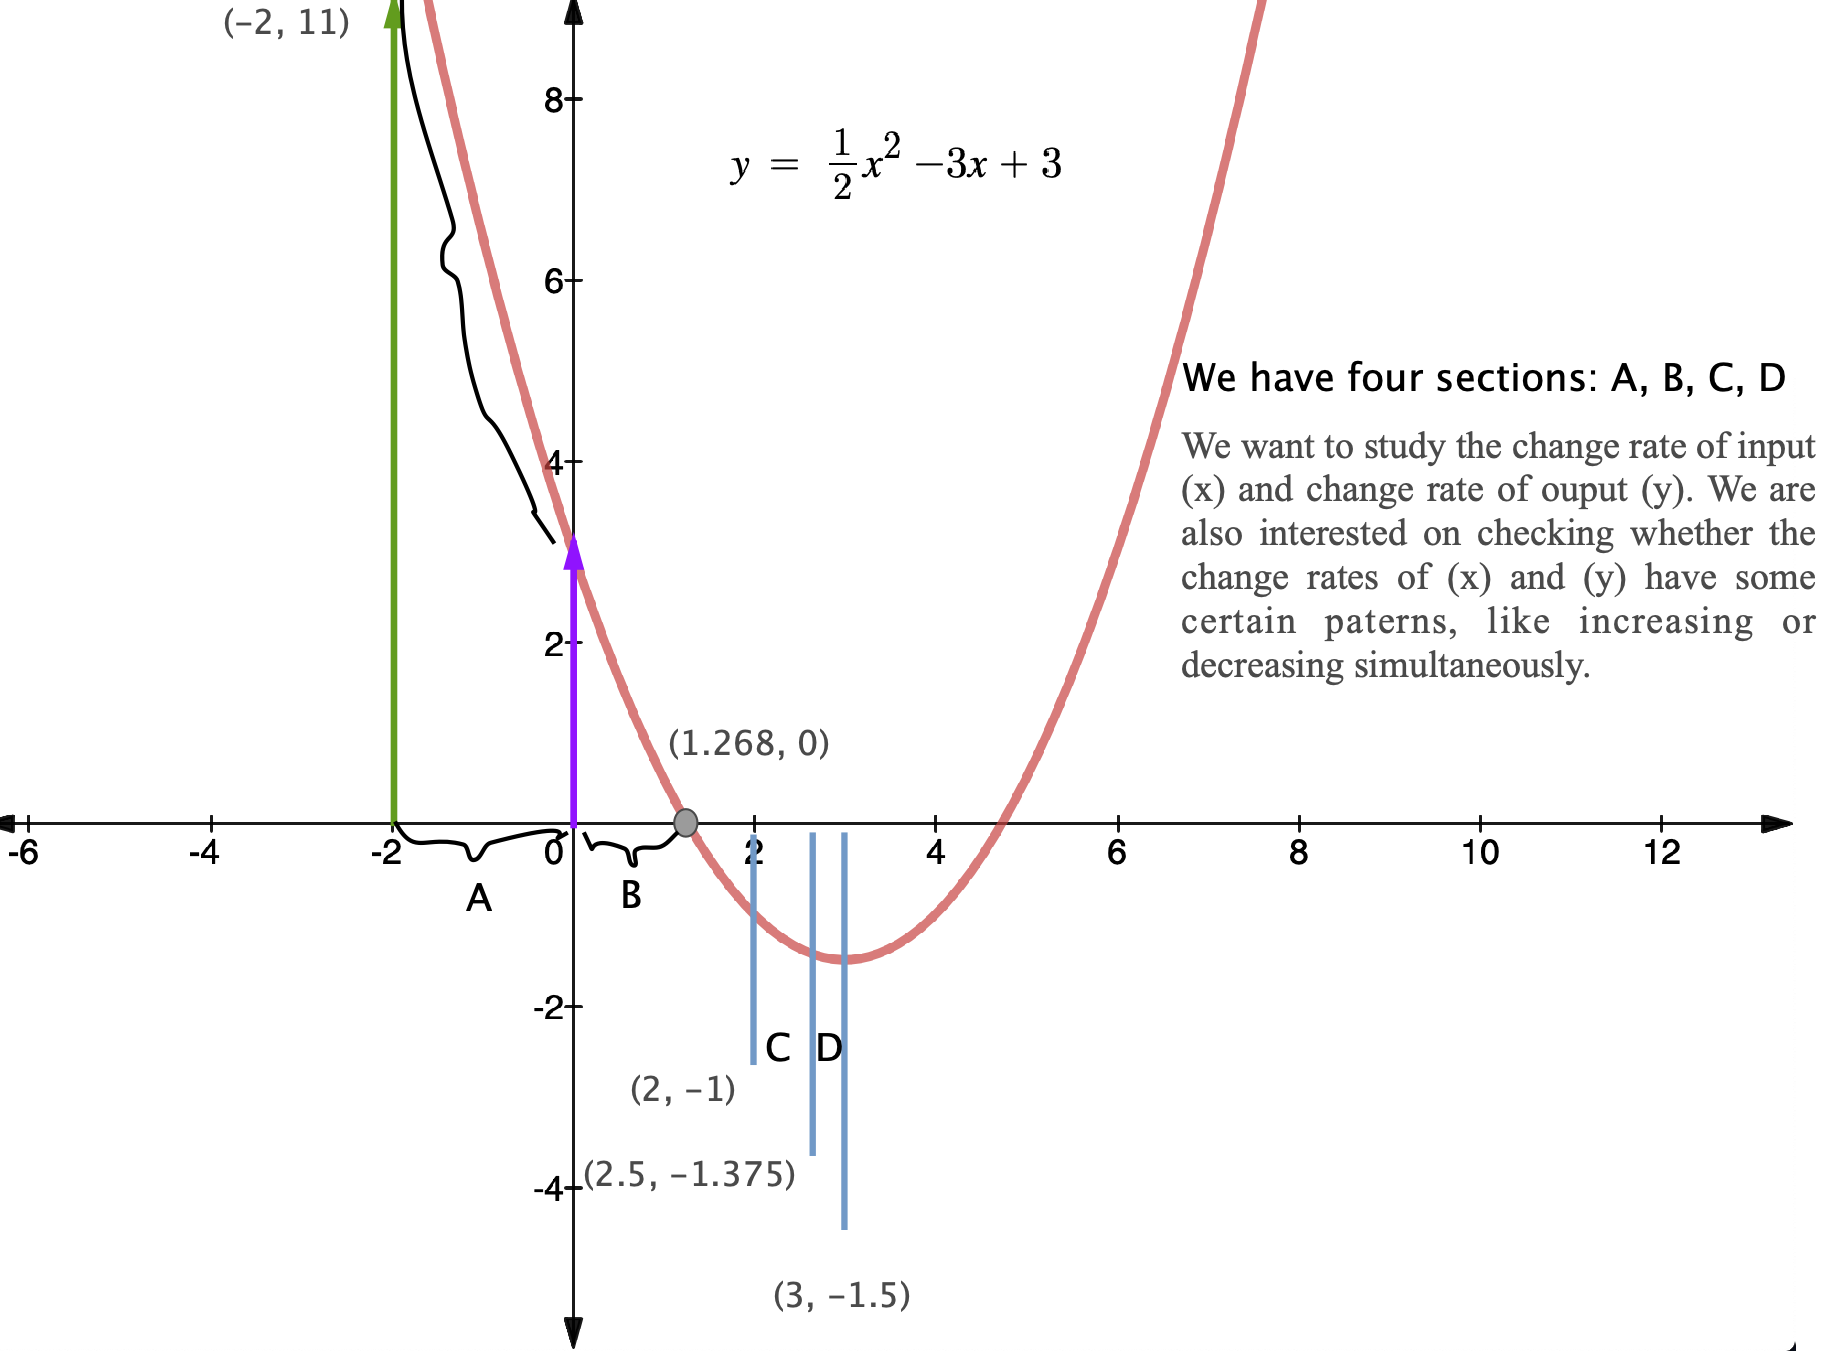
\includegraphics[width=0.7\textwidth]{gradientEg}
  \caption{Gradient Visualisation}
\end{figure}

Again, the derivative is not just about the measurement of change of input and output, it also reflects the sensitivity of those changes. Take a look the figure 1.1, tell me where both input ($x$) and output ($y$) are changing fast, and where both input ($x$) and output ($y$) are changing slowly\footnote{If we assume that speed of changing is measured by the difference between two values.}.

From the figure 1.1, we can see that in section A, both input ($x$) and output ($y$) are changing quite fast by measuring the differences. When it comes to section C and D, the changing rates for input-$x$ and output-$y$ are decreasing simultaneously. We also say that input $x$ and output $y$ have the same \textbf{convergence rate} intuitively\footnote{This is not formal mathematical definition.}. For the \textbf{supervised learning} in \textit{machine learning}, it starts to do optimization with the tool of convergence rate.

Now, let's check the formal definition of derivative. The slope $m$ of the secant line is the difference between the y values of these points divided by the difference between the x values, that is,
\begin{align*}
  m = \frac{\Delta f(x)}{\Delta x} = \frac{f(x+h) - f(x)}{(x+h) -x} = \frac{f(x+h)-f(x)}{h}
\end{align*}
Geometrically, the limit of the secant lines is the tangent line. Therefore, the limit of the difference quotient as $h$ approaches zero, if it exists, should represent the slope of the tangent line to $(x, f(x))$. This limit is defined to be the derivative of the function $f$ at $x$:
\begin{align*}
  f'(x) = \lim_{h\to 0} \frac{f(x+h) - f(x)}{h}
\end{align*}

With the riview of defintion of derivative, we are ready to apply the so called \textbf{gradient descent} algorithm to find the minimum of a function.
\begin{definition}
  Gradient descent is a first-order iterative optimization algorithm for finding the minimum of a function.
\end{definition}

Let's disentangle the convergence rate for the function $y= \frac{1}{2}x^2 - 3x + 3$ in figure 1.1 by presenting the following figure and table:
\begin{figure}[H]
  \centering
  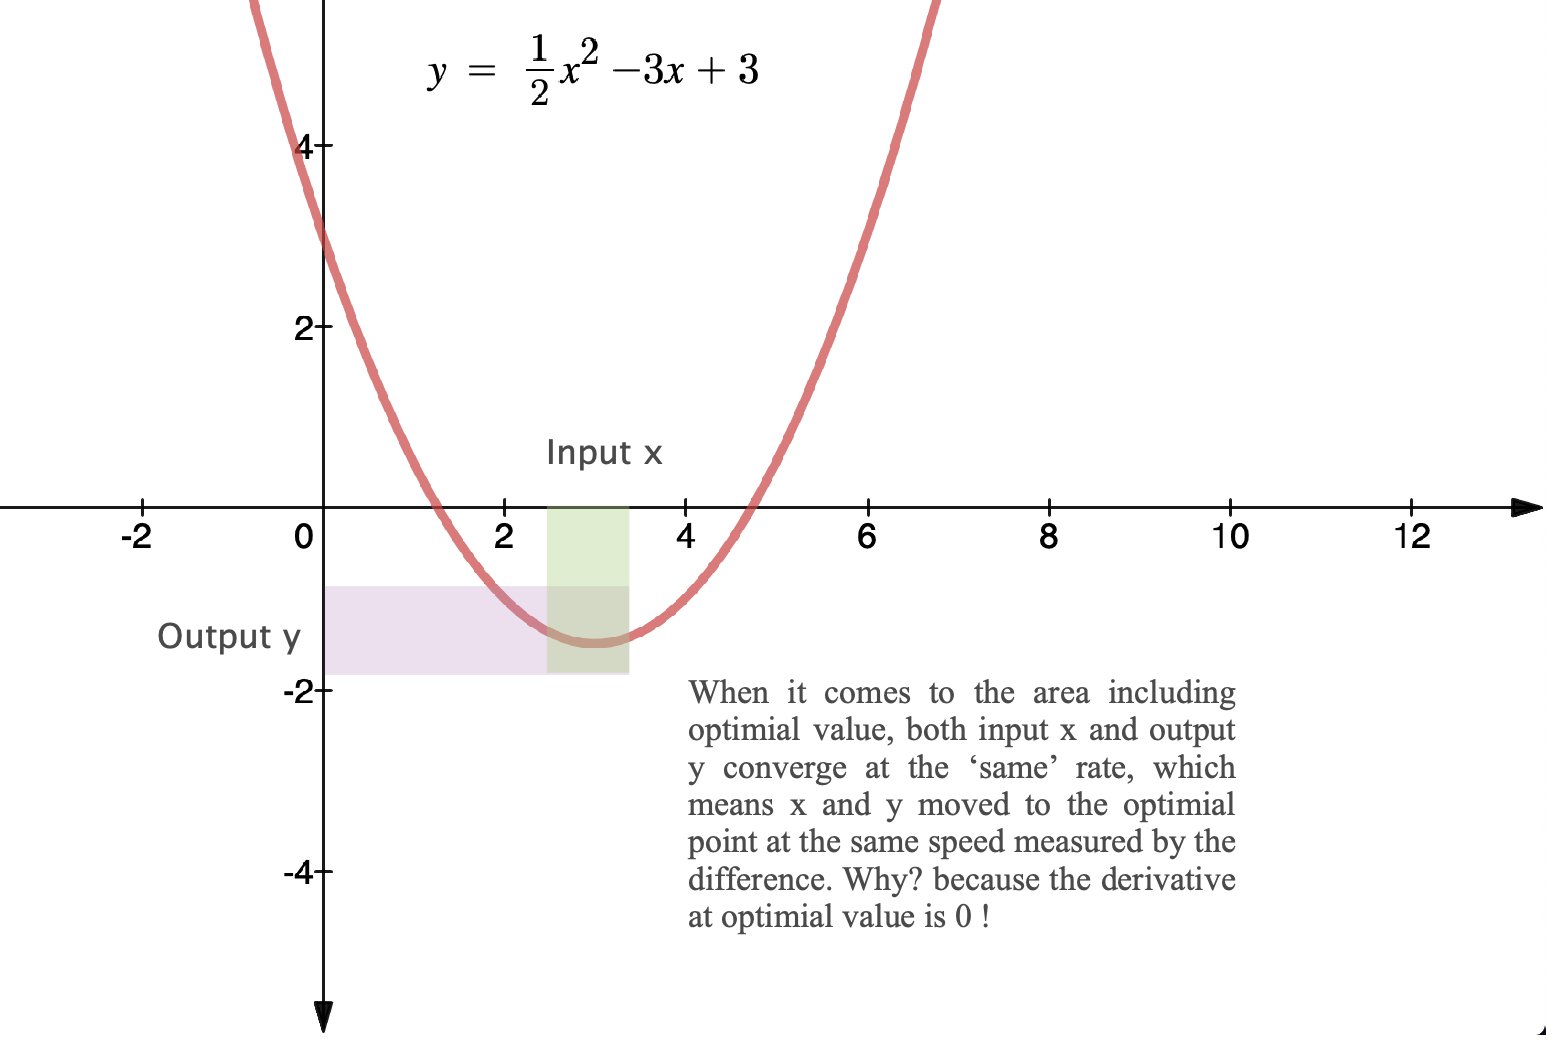
\includegraphics[width = 0.7 \textwidth]{gradientEg2}
\end{figure}
{\footnotesize
\begin{table}[H]
  \centering
  \caption{Show the gradient descent step by step}
  \begin{tabular}{lcccc}
    \hline
    \hline
    Section & Points & Change of input($x$) & Change of ouput ($y$) & Convergence ratio  \\
    \hline
    A & $(-2, 11)$ & \\
    & $(0,0)$ & 2 & 11 & $11/2 = 5.5$ \\
    \hline
    B & $(0,0)$ & \\
    & $(2, $-$1)$ & 2 & 1 & $1/2 = 0.5$ \\
      \hline
    C & $(2, $-$1)$ &  \\
    & $(2.5, $-$1.375)$ & 0.5 & 0.375 & $0.375/0.5 = 0.75$ \\
    \hline
    D & $(2.5, $-$1.375)$ & \\
    & $(3, $-$1.5)$ & 0.5 & 0.125 & $0.125/0.5 = 0.25$ \\
    \hline
    \multicolumn{5}{c}{$\cdots$} \\
    \hline
    & $(2.9, $-$1.49499)$& \\
    & $(2.95, $-$1.49875)$ & 0.05 & 0.00376 & $0.00376 /0.05 = 0.075$  \\
    \hline
    \multicolumn{5}{c}{$\cdots$} \\
    \hline
    & $(2.98, $-$1.499799)$& \\
    & $(2.99, $-$1.499950)$ & 0.01 & 0.000151 & $0.00376 /0.05 = 0.00151$  \\
    \hline
    \multicolumn{5}{c}{we have learning rate $\alpha$ to scale the convergence rate = 1} \\
    \hline
  \end{tabular}
\end{table}
}

\textbf{Markup:} it's all about simultaneous moving of input ($x$) and ($y$).

\section{A Mathematical example}

Now, we will employ the gradient descent\footnote{Review the definition, it's an algorithm.} to find the minimum value for the function in section 1:
\begin{align*}
  f(x) = \frac{1}{2} x^2 - 3x + 3
\end{align*}

The intuition of using gradient descent is that we are trying to iterate the change rate of input $x$ by tracing the change rate of output $y$. To do this, we need the help from the derivative of the function. Here is the Python code:
\begin{lstlisting}
  # Gradient Descent: mathematical example
  # @ Michael


  # define function
  def qudraticfun(x):
      y = 1/2 * x**2 - 3 * x + 3
      return(y)


  # define the derivative
  def qudraticder(x):
      yprime = x - 3
      return(yprime)


  # find the minium numerically

  update_x = 0  # most time we start it from zero
  alpha = 0.01  # learning rate
  tolerate_rule = 1  # initialize the tolerate rule for stopping iterating
  max_iters = 10000  # set the maximum iterative number

  i = 0  # interation counting index
  while tolerate_rule >= 0.00001 and i <= max_iters:
      start_x = update_x  # set the starting value
      update_x = start_x - alpha * qudraticder(start_x)
      tolerate_rule = abs(update_x - start_x)

  print("The minimum value is", qudraticfun(update_x),
        "when x is equal to", update_x)

  # The minimum value is -1.4999995136117308 when x is equal to 2.999013705653870
\end{lstlisting}

\section{A Machine Learning Example}

























\newpage
\bibliography{/Users/Michael/Documents/MachineLearning/ML.bib}
\bibliographystyle{apalike}
\end{document}
